\documentclass[../../../main.tex]{subfiles}
\begin{document}
From the attempts commented on in \textcolor{red}{Section X} arises the following question: 

\textbf{Is there a way to group the points of the base to find an apex, from those groups, that satisfies all the restrictions?}

From this question, it can be deduced that, to answer it, a way of grouping the points of the base must first be found.
This grouping task should result in a surface where all points are joined using closed lines that cannot cross. 
In other words, a different simple\footnote{A  polygon is simple if it is single-connected and the bordering line does not intersect itself. Additionally, a polygon is single-connected if its border forms a single, closed line.} polygons without gaps or overlaps should be used. 
It is, obviously, a tessellation task.

Several tessellation algorithms tessellate 2D or 3D surfaces, but the Delaunay triangulation\footnote{In computational geometry, a Delaunay triangulation of a set of points in the plane subdivides their convex hull into triangles whose circumcircles do not contain any of the points.} was chosen due to it maximizes the size of the smallest angle in any of the triangles, and tends to avoid sliver triangles.
Moreover, Delaunay triangulation assures the connection between all the points and does not create or delete points.
The majority of the triangulation algorithms aim to subdivide a geometric surface into non-overlapping triangles by joining the vertices of the hull.
In addition, it is widely implemented in many Python libraries.
In this work, the function \textit{Delaunay} of the submodule \textit{spatial} of the \textit{SciPy} library is used\footnote{\href{https://docs.scipy.org/doc/scipy/reference/generated/scipy.spatial.Delaunay.html}{scipy.spatial.Delaunay}}.
Given a set of \textit{n} points, this function returns, among other things, a list of the simplices\footnote{In geometry, a simplex, plural: simplices, is a generalisation of the notion of a triangle or tetrahedron to arbitrary dimensions. A 2D-simplex is a triangle.} in the triangulation.
And these simplices will be used as the groups of points from the base mentioned above, from which to try to find a vertex, for each of them, that satisfies all the restrictions. 
An example of the tessellation of a set of points of the base of a cylinder with a diameter of 3 mm is shown in \textcolor{blue}{Figure} \ref{fig:tessellation}.

\begin{figure}[!htbp]
    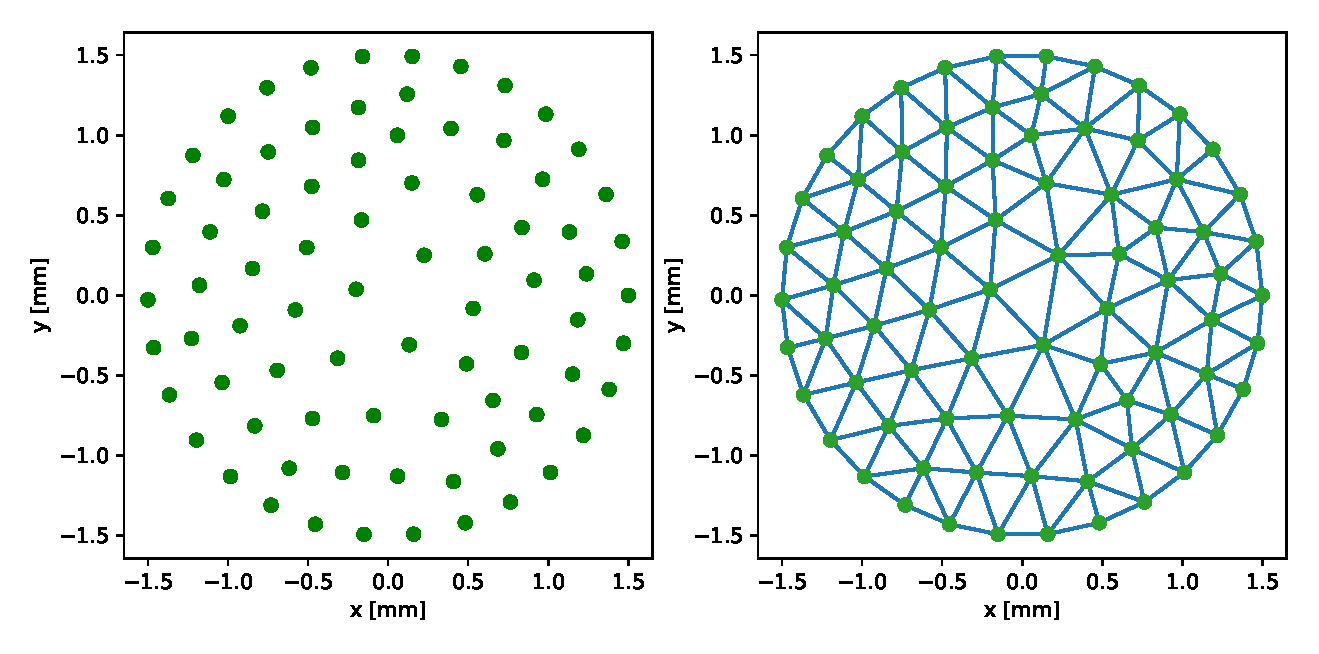
\includegraphics[width=1\textwidth]{imgs/tessellation.eps}
    \centering
    \caption{Example of tessellation of a set of points of the base of a cylinder with a diameter of 3 mm}
    \label{fig:tessellation}
\end{figure}


Once the tessellation is obtained, the next step is to find a vertex for each of the simplices that satisfies all the restrictions, thus obtaining a pyramid for each of the simplices.
The main restriction is that the angle between each edge and the base must be at least 45 degrees to ensure stability.
To guarantee this condition, an optimisation algorithm is used to find the vertex that minimises the angle between the edges and the base.

To accomplish this, given N points representing the points of the base of the pyramid, the objective is to find the point that minimizes the inner product between the vector formed by each base point and this point, and the vector normal to the horizontal plane, $\vec{n_z} = (0,0,-1)$.
However, if a minimum point is to be obtained when $\theta = 45^\circ$, it is not sufficient to minimise the inner product, but a function that makes this product minimum when $\theta = 45^\circ$ must be minimised.
Since the inner product between two vectors is equal to the product of the magnitudes of the vectors and the cosine of the angle between them (\textcolor{blue}{Equation} \ref{eq:inner_product}), the angle between the vectors can be calculated as the arccosine of the inner product divided by the product of the magnitudes of the vectors (\textcolor{blue}{Equation} \ref{eq: angle}).
So, the function to optimize, $g(\vec{a}, \vec{b})$ is the arccosine of the inner product between the vector formed by each base point and the point to find, and the vector normal to the horizontal plane, minus 45 degrees (\textcolor{blue}{Equation} \ref{eq:opt_func}).
This ensures that the minimum value of this function will be at the minimum allowable edge angle. 
Therefore, the position of the vertex obtained will be that which guarantees that the edges of the pyramid have an angle as close to 45 degrees as possible.


\begin{equation}
    \vec{a} \cdot \vec{b} = \lVert \vec{a} \rVert \lVert \vec{b} \rVert \cos(\theta)
    \label{eq:inner_product}
\end{equation}


\begin{equation}
    \theta = \arccos(\frac{\vec{a} \cdot \vec{b}}{\lVert \vec{a} \rVert \lVert \vec{b} \rVert})
    \label{eq:angle}
\end{equation}

\begin{equation}
    g(\vec{a}, \vec{b}) = \arccos(\frac{\vec{a} \cdot \vec{b}}{\lVert \vec{a} \rVert \lVert \vec{b} \rVert}) - 45
    \label{eq:opt_func}
\end{equation}


This function, $g(\vec{a}, \vec{b})$ (\textcolor{blue}{Equation} \ref{eq:opt_func}), must be evaluated for each of the N points of the base. 
But, the apex to be found must guarantee that this function is minimal for each of the points of the base.
So, it cannot be evaluated separately for each of the points of the base, but for all of them at the same time.
Then, the objective function to minimise would be the sum of the result of the function for each of the points of the base (\textcolor{blue}{Equation} \ref{eq:opt_func_sum}).
Since the inner product is known to be with respect to the horizontal plane, and its normal vector is known, the only unknowns are the coordinates of the point to be found. 
Leaving $f(\vec{x})$ and $g(\vec{x})$ as a functions of the coordinates of the point to be found, $\vec{x} = (x, y, z)$.

\begin{equation}
    f(\vec{x}) = g_1(\vec{x}) + g_2(\vec{x}) + ... + g_N(\vec{x})
    \label{eq:opt_func_sum}
\end{equation}


To simplify the problem, the coordinates of the point to be found are limited to a certain range. 
Concerning the x-dimension, the range of values is limited by the maximum and minimum x-dimension value of the coordinates of all points in the base. The same is true for the y-dimension. 
For the z-dimension, the minimum value it can take is the minimum value of z of the coordinates of the basis.
And the maximum will be equal to the sum of the minimum value of z and the width of the x-dimension range.
Then, the optimisation problem to be solved is formulated in \textcolor{blue}{Equation} \ref{opt:opt_problem}.
Where $x_{n}$, $y_{n}$, and $z_{n}$ are the coordinates of the n-th point of the base, and $x_{min}$, $x_{max}$, $y_{min}$, $y_{max}$, $z_{min}$, and $z_{max}$ are the minimum and maximum values of the x, y, and z dimensions, respectively.



\begin{mini}
    {x, y, z}{\sum_{1}^{N} \arccos(\frac{z_n - z}{\lVert \vec{(x_n - x, y_n - y, z_n - z)}\rVert · \lVert \vec{n_z} \rVert}) - 45}{}{}
    \addConstraint{x}{\in [x_{min}, x_{max}]}
    \addConstraint{y}{\in [y_{min}, y_{max}]}
    \addConstraint{z}{\in [z_{min}, z_{min} + (x_{max} - x_{min})]}
    \label{opt:opt_problem}
\end{mini}


To solve this optimisation problem, the \textit{SciPy} optimisation module, \textit{scipy.optimize}, was used at first, specifically the \textit{minimise} function\footnote{\href{https://docs.scipy.org/doc/scipy/reference/generated/scipy.optimize.minimize.html}{scipy.optimize.minimize}}.
But it was found that it was faster to solve the problem by using high-dimensional vectors.
So, using the library \textit{NumPy}, a 4-dimensional array was created by a meshgrid of the x, y, and z dimensions from three fifteen-point equispaced arrays that covered the x, y, and z dimensions ranges.
Then, the function to minimise was evaluated for each of the points of the mesh grid, and the minimum value that the function was selected.
To avoid situations where the minimum value is found in a position where any of the edges does not meet the angularity condition, a penalty was applied to those points that leave any edge with an angle lower than 45 degrees.
An example of the result of the optimisation process is shown in \textcolor{blue}{Figure} \ref{fig:optimization}.
This figure shows in black an arbitrary base formed by the points (0,0,0), (1,0,0), (0,1,0), and in colour the value of the function, varying according to the value. 
The optimal point found is shown as a red star.

\begin{figure}[!htbp]   
    \centering
    \includegraphics[width=0.7\textwidth]{opt_func.png}
    \caption{Example of the result of the optimisation process}
    \label{fig:optimization}
\end{figure}

If this process is repeated for each of the simplices of the tessellation, a pyramid will be obtained for each of them. 
An example of the result of this process is shown in \textcolor{blue}{Figure} \ref{fig:pyramids}.
As can be seen in the figure, each of the apexes found is connected to some points of the base, making them connected to the base by at least 3 edges.
This process guarantees that the structure is fully connected and that the edges meet the angularity condition.

\begin{figure}[!htbp]
    \centering
    \includegraphics[width=0.7\textwidth]{imgs/pyramids.png}
    \caption{Example of the result of the process of finding the apex of the pyramids for each of the simplices of the tessellation of the base of a cylinder with a diameter of 3 mm.}
    \label{fig:pyramids}
\end{figure}

Now, new points created, the apexes, can be treated as new points of the following base, and the process can be repeated to find new apexes and grow the structure. 
But, as it can be seen in the \textcolor{blue}{Figure} \ref{fig:optimization}, the apexes created do not lie on the surface of the cylinder, but they are inside it.
Thus, if the new points are tessellated to start again the finding of the vertices, the new vertices will converge towards the centre of the volume as the new vertices in each layer will always be inside those of the previous one.
To avoid that, and to maintain the original shape of the volume, the new points must be in some way connected to the surface of the volume.


To do that, initially, from all the new points, the mean height was calculated, and a section of the shell was extracted at that height.
This brings the problem that the shell is not really a continuous surface but a set of points. 
It is not possible to extract a section of it at a desired height. 
Because there may be no points of the shell at that height, or not enough points to represent the shell section.
Then, instead of extracting a section of the shell at a certain height, from this mean height, the shell points whose heights lie within a range centred on the mean height are extracted. 
To calculate the width of this range, the characteristic distance of the shell points has been calculated by calculating the cumulative sum of the distance of each point to its nearest neighbour and dividing it by the number of points (\textcolor{blue}{Equation} \ref{eq:char_dist}), 

\begin{equation}
    d = \frac{\sum_{1}^{N} \lVert \vec{p_n - p_{n+1}} \rVert}{N}.
    \label{eq:char_dist}
\end{equation}

Where $d$ is the characteristic distance, $N$ is the number of points, and $p_n$ is the n-th point of the shell.
Then, the width of the range is calculated as the characteristic distance multiplied by a proportionality factor, $\kappa$, to vary the width of the range.
This was done because using the characteristic distance as the width of the range resulted in extractions with too many points, and the section was saturated with points.
The ideal section would have its points distributed uniformly along the perimeter of the shell, but the extraction of the points is not uniform, and the points are grouped in some areas.
But by reducing the width of the range, the number of points extracted is reduced, and the section is more uniform.
Although if the width of the range is too low, the section may not be continuous, and the points may not be connected.
An example of how the width of the range affects the number of points extracted is shown in \textcolor{blue}{Figure} \ref{fig:shell_points}.
Finally, it was observed that a width range of half of the characteristic distance, $\kappa = 0.5$, was the most suitable to extract the shell points.

\begin{figure}[!htbp]
    \centering
    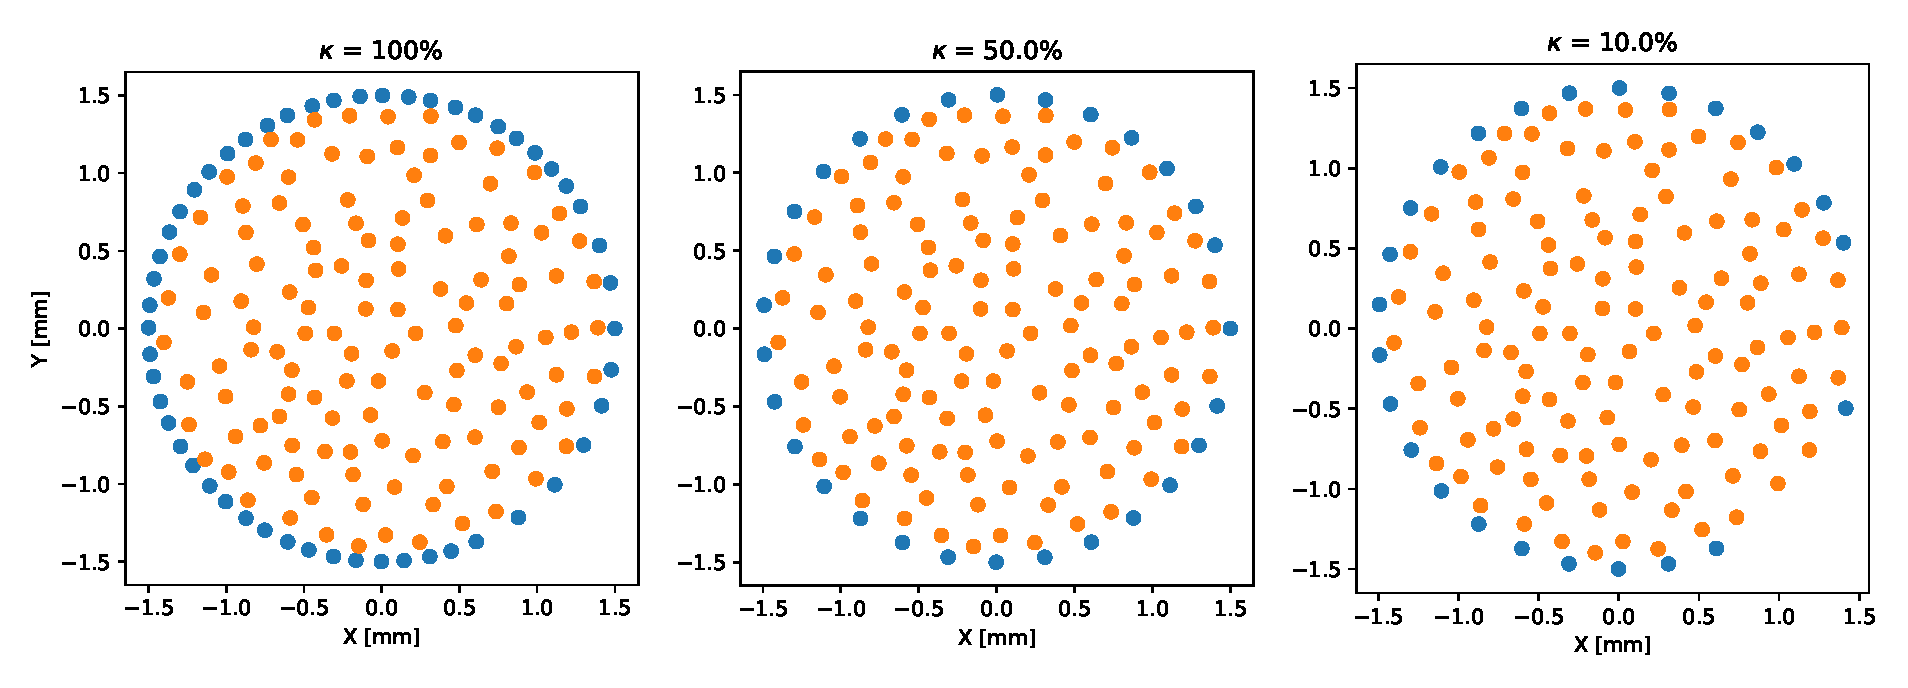
\includegraphics[width=1\textwidth]{imgs/shell_points.eps}
    \caption{An example of how the wider the range for extracting shell points will affect the number of points extracted. Low values of proportionality can lead to extractions with so few points that the section is not continuous. Orange points represent the apexes created, and the blue points represent the points of the shell.}
    \label{fig:shell_points}
\end{figure}

Although it is true that by reducing the width of the range to be considered, it is possible to control the number of points to be extracted and thus obtain a uniform section. 
It may be that, because the surface mesh is not regular or homogeneous, it may appear that a uniform section is being obtained when the section is observed using its projection.
But in the three-dimensional space, this may not be the case, and more points are being taken than desired, highlighting the lack of control over the extraction of the section. 
In the \textcolor{blue}{Figure} \ref{fig:shell_points_3}, an example of this situation is shown. 
The section from the middle image of the \textcolor{blue}{Figure} \ref{fig:shell_points} is represented from a three-dimensional view.
And can be observed that there are some points that belong to the upper layers that should not be considered in the current section.
As the $\kappa$-factor cannot be adapted in each layer and there is no way of knowing whether the section being extracted is ideal or not, this excess of points is something that would have to be dealt with during the process of structure generation. 
These points, being too close to each other in their projection, will cause very narrow triangles to appear in the next triangulation and are undesirable as they increase the local density of edges and may cause the separation condition not to be fulfilled in some of them. 
An example of this narrow triangle can be seen in the right image of the \textcolor{blue}{Figure} \ref{fig:shell_points_2}.

\begin{figure}[!htbp]
    \includegraphics[width=0.7\textwidth]{imgs/shell_points_3.png}
    \centering
    \caption{Representation of the shell points extracted by taking the average height of the points. Orange points represent the hull points of the points from the \textcolor{blue}{Figure} \ref{fig:shell_points}, and the blue points represent the points extracted from the shell.}
\label{fig:shell_points_3}
\end{figure}


Moreover, this solution for connecting the new points to the points on the surface has an additional problem related to extracting points from the shell whose heights lie within a range centred on the average height, and that is that the points extracted are not related to the design parameters.
This could lead, for example, to situations where the pore size is so large that the number of points extracted from the shell is too high compared to the number of vertices created.
Leaving areas where the points of the shell have no closer points to join and are forced to join inner points during the triangulation.
Thus, the next layer of vertices will be so close to each other that it will be impossible to meet the distance condition for these points.
In the top right of the right image in \textcolor{blue}{Figure} \ref{fig:shell_points_2}, and in the bottom, an example of this situation is shown.

\begin{figure}[!htbp]
    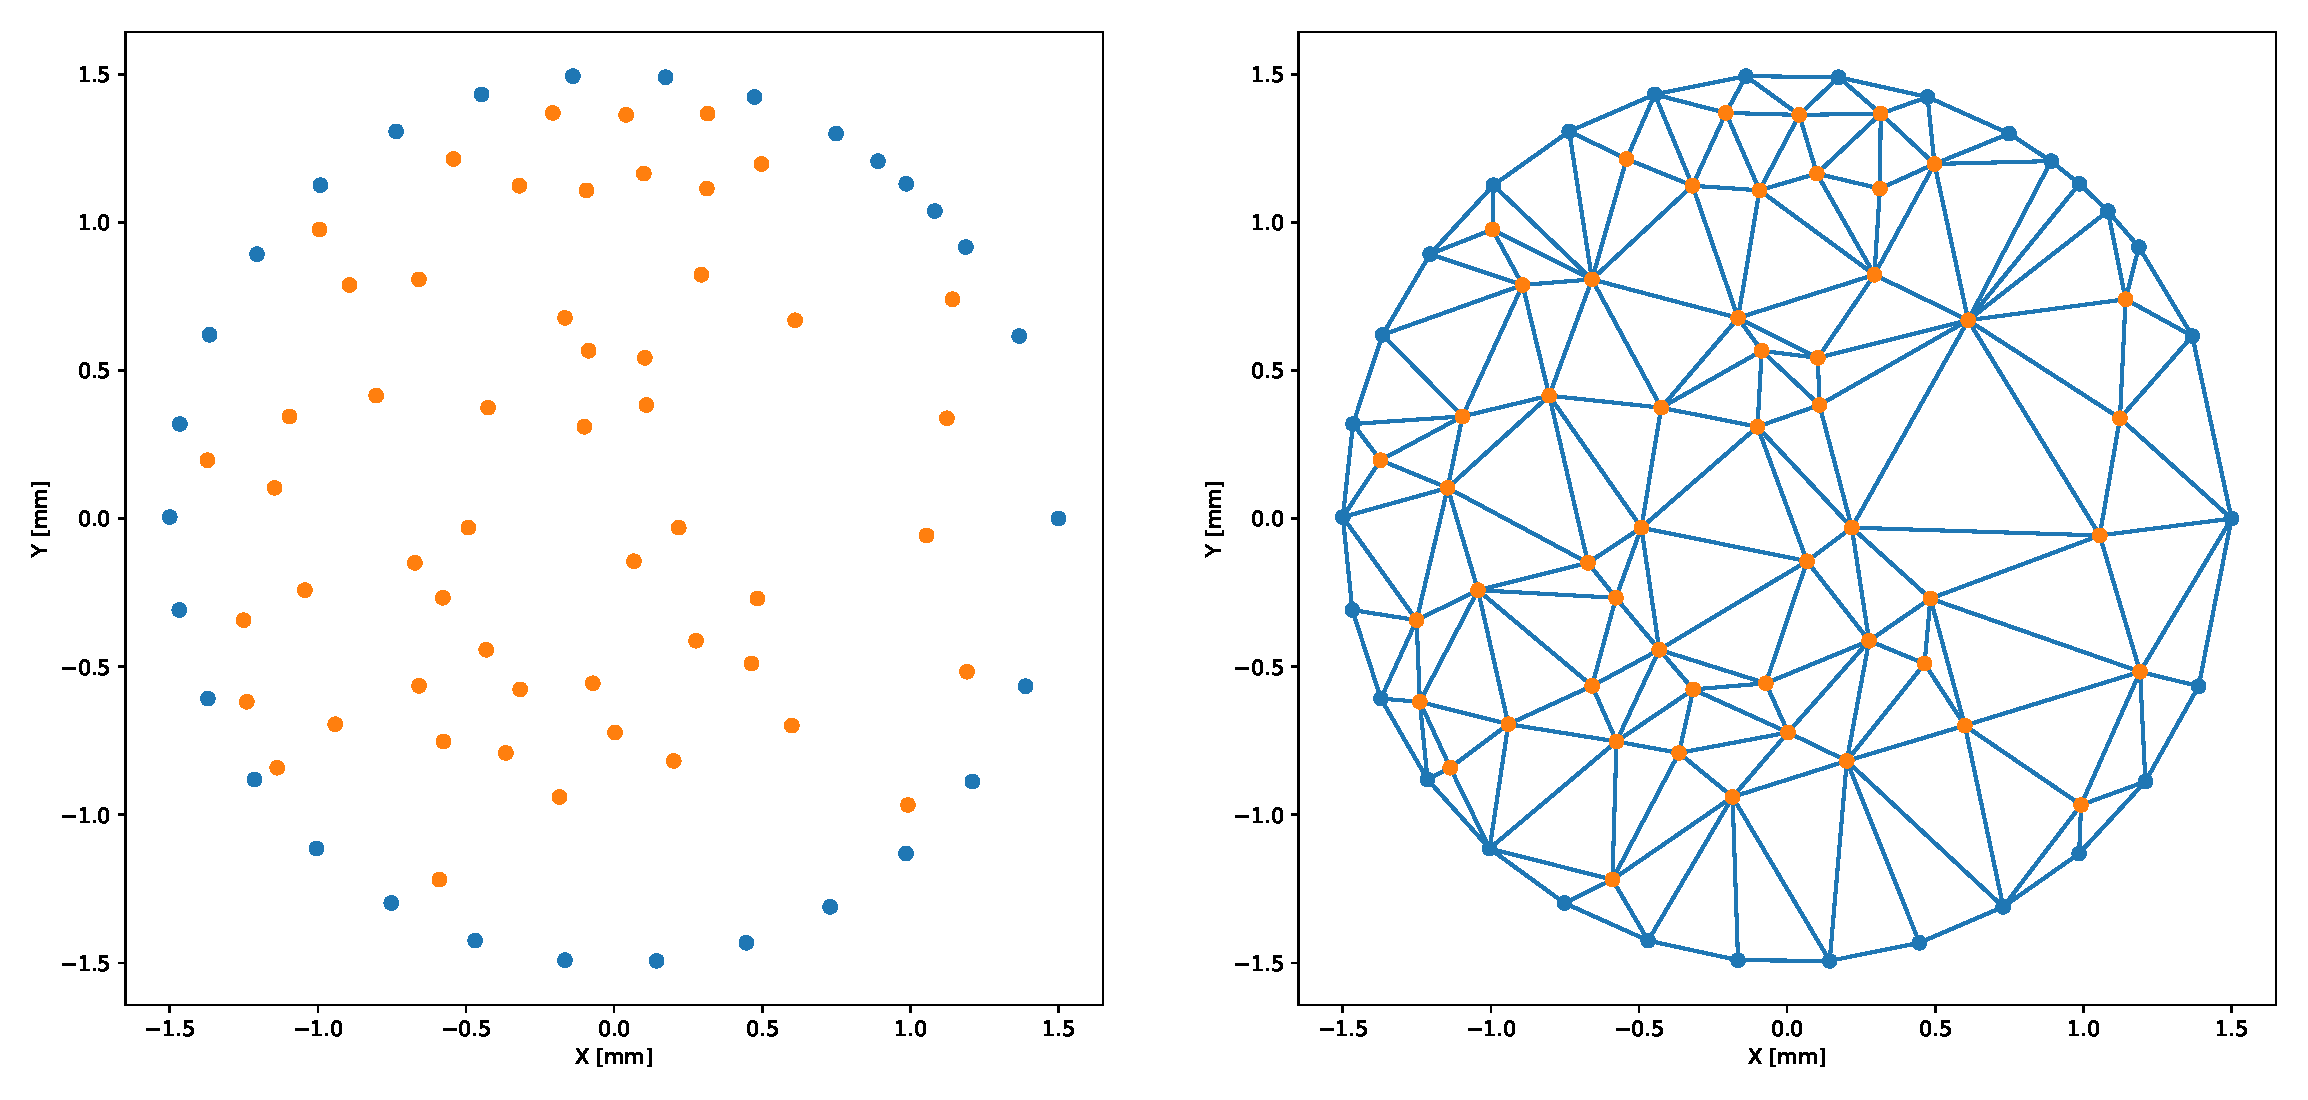
\includegraphics[width=1\textwidth]{imgs/shell_points_2.eps}
    \centering
    \caption[An example of how the number of points extracted from the shell can be too high compared to the number of apexes created and the resulting Delaunay tessellation for this set of points.]{An example of how the number of points extracted from the shell can be too high compared to the number of apexes created \footnotemark and the resulting Delaunay tessellation for this set of points.}
\label{fig:shell_points_2}
\end{figure}
\footnotetext[6]{This image was created from the central image in \textcolor{blue}{Figure} \ref{fig:shell_points} by randomly removing the 80\% of the apexes.}

This can be solved if, instead of extracting the points from the shell whose heights lie within a range centred on the average height, the closer points to the outer vertices are extracted. 
Thus, points extracted from the shell will be controlled by the number of vertices created, which in turn is related to the pore size.
In the \textcolor{blue}{Figure} \ref{fig:shell_points_4}, an example of this change is shown. 
It can be seen that now the points of the shell are not in a slice but are located near the outer vertices, and the number of points is smaller.
In the \textcolor{blue}{Figure} \ref{fig:shell_points_5}, the Delaunay tessellation of the points extracted from the shell by both methods is compared.
The differences are slight, but it can be seen that the number of narrow triangles is reduced significantly.
Using this approach may seem that the shape of the volume section loses definition, but it is necessary to remember that the lines between the points will not be present in the three-dimensional model, but are the result of the triangulation of the points and are added to make it easier to understand the process of generating the structure.
As these points are points that belong to the surface of the volume, the shape of the volume will be maintained, and the structure will be connected to the surface.
In fact, the only things that are part of the structure are the points shown in the images. 
The triangles are to be understood as elements that indicate which points will join the following vertices.
It is therefore necessary for the reader to bear this in mind when looking at the images.


\begin{figure}[!hbtp]
    \includegraphics[width=0.7\textwidth]{imgs/shell_points_4.png}      
    \centering
    \caption{Result of the vertex search algorithm for the base points, in black: (0,0,0), (1,0,0,0) and (0.5,0.5,1). The vertex obtained is shown in red and is located at the point (0,0.5,3.1).}
\label{fig:shell_points_4}
\end{figure}


\begin{figure}[!hbtp]
    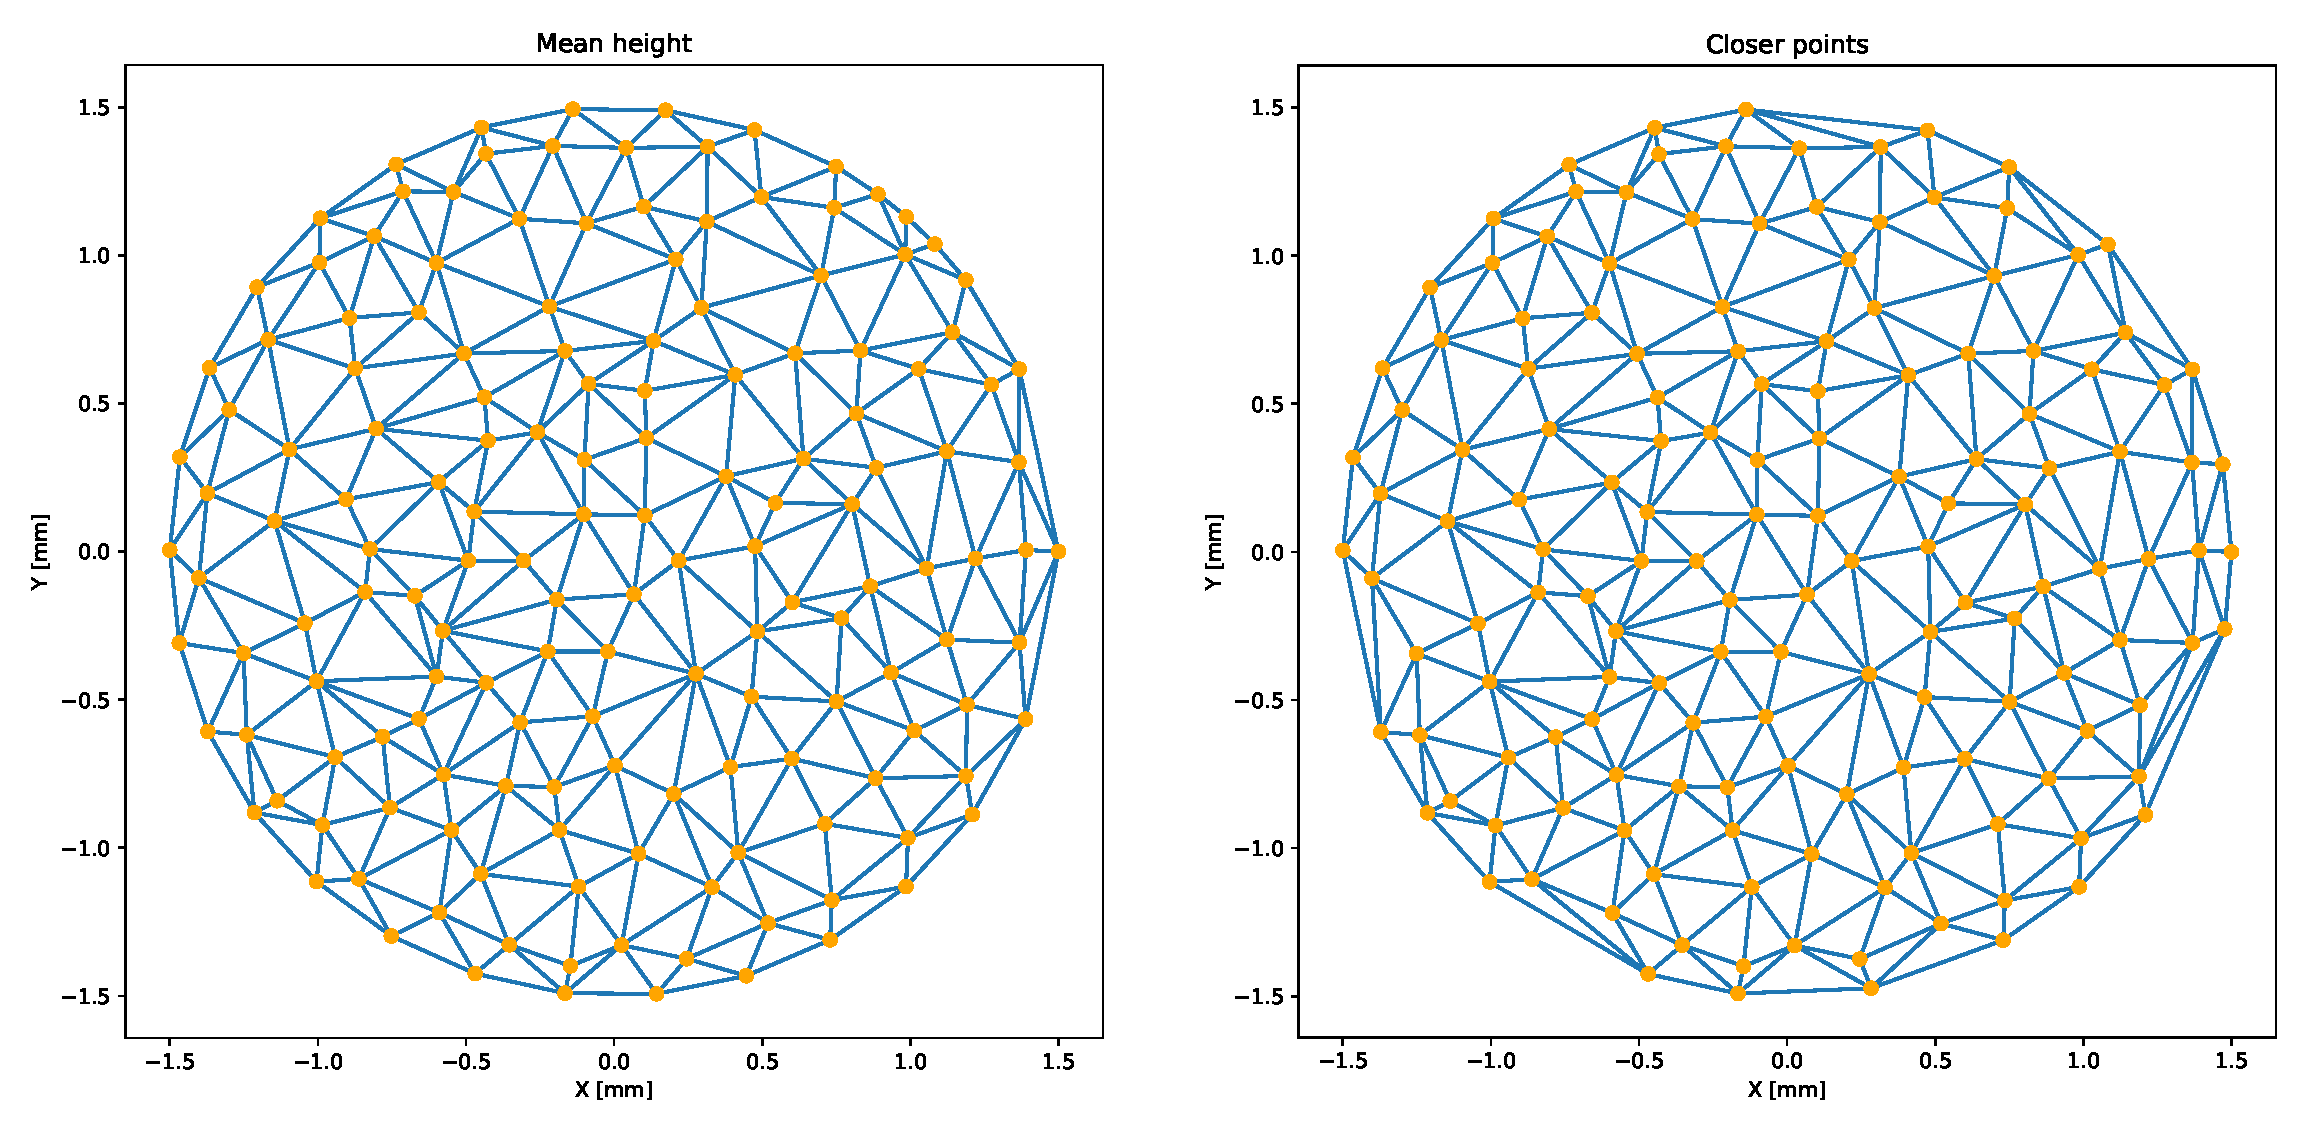
\includegraphics[width=0.8\textwidth]{imgs/shell_points_5.eps}
    \centering
    \caption{Comparison between the Delaunay tessellation of the points extracted from the shell by taking the average height of the points (right) and the points extracted from the shell by taking the closest points to the outer vertices (left).}
\label{fig:shell_points_5}
\end{figure}


Up to this point, it has been possible to group a set of points using triangulation, it has been possible to generate, from these triangles, the optimum vertex that fulfils the established conditions and, subsequently, those points of the surface that are closest to each of the outermost generated vertices are joined to the surface of the volume by selecting those points of the surface that are closest to each of the outermost generated vertices. 
This process closes the flow of each iteration. 
Therefore, a priori, if this process were repeated until the upper base of the volume is reached, the desired structure would be obtained.

However, the process is not as simple as it seems. 
The main problem is that the number of points generated over the iterations is not constant, but increases with each iteration. 
According to Euler's characteristic ($\chi$), there is an invariant relationship between the topological structure of a domain. 
Euler proved that for a convex polygon:
\begin{equation}
   \chi =  V - E + F = 1
    \label{eq:euler}
\end{equation}
Where V is the number of vertices, E is the number of edges, and F is the number of faces. 
In the case of triangulations, every triangle (face) is connected to another triangle by each of its edges, and each triangle has three edges. Then: 
\begin{equation}
    2E = 3F
    \label{eq:edges}
\end{equation}
If \textcolor{blue}{Equation} \ref{eq:edges} is substituted into \textcolor{blue}{Equation} \ref{eq:euler}, the following is obtained:
\begin{equation}
    F = 2(V - 2)
    \label{eq:euler_2}
\end{equation}
But in the case of planar triangulations, the edges of the hull are only connected to one triangle. 
Let H be the number of edges of the hull; then there are $ E-H$ internal edges. 
These internal edges are shared by two triangles, and each triangle has three edges. 
Then, \textcolor{blue}{Equation} \ref{eq:edges} can be rewritten as:

\begin{equation}
    2(E - H) + H = 3F
    \label{eq:edges_2}
\end{equation}

If the \textcolor{blue}{Equation} \ref{eq:edges_2} is substituted into \textcolor{blue}{Equation} \ref{eq:euler}, the following is obtained:

\begin{equation}
    F = 2(V - 1) - H
    \label{eq:euler_3}
\end{equation}

Where, in fact, F is the number of triangles that given V vertices and H edges of the hull will be generated by the triangulation. 
Since the number of vertices will always be greater than the number of points in the hull, it can be seen that the number of triangles generated will be $F \approx 2V$. 
As a new vertex is generated for each triangle, the number of vertices generated in the next layer is F. 
It follows that the number of vertices is approximately doubled in each layer. 
This can be seen in \textcolor{blue}{Figure} \ref{fig:euler} where the number of simplices and points is shown for the first four layers. 
It is then easy to deduce that the density of the structure is not constant, but increases with the Z-axis. 
Moreover, this density gradient would make it impossible to keep the design parameters and meet the conditions.
Therefore, is it necessary to implement a mechanism to control the number of points generated in each layer, or the triangles instead.


\begin{figure}[H]
    \centering
    \begin{subfigure}[h]{0.45\textwidth}
        \centering
        \includegraphics[width=\textwidth]{imgs/iteration_0.png}
        \caption{F: 126, V: 79, H: 30}
    \end{subfigure}
    \begin{subfigure}[h]{0.45\textwidth}
        \centering
        \includegraphics[width=\textwidth]{imgs/iteration_1.png}
        \caption{F: 279, V: 155, H: 29}
    \end{subfigure}
    \begin{subfigure}[h]{0.45\textwidth}
        \centering
        \includegraphics[width=\textwidth]{imgs/iteration_2.png}
        \caption{F: 586, V: 309, H: 30}
    \end{subfigure}
    \begin{subfigure}[h]{0.45\textwidth}
        \centering
        \includegraphics[width=\textwidth]{imgs/iteration_3.png}
        \caption{F: 1201, V: 617, H: 31 }
    \end{subfigure}
        \caption{Topological structure of the first four layers of the structure.}
        \label{fig:euler}
\end{figure}

\end{document}